% Individual-Based Modeling (IBM)
%
% Advanced Project I - Jacobs University Bremen
% Supervisor: Dr. Stefan Kettemann
%
% Created on May 29, 2019
%
% Authors:
%   Ralph Florent <r.florent@jacobs-university.de>
%   Davi Tavares <davi.tavares@leibniz-zmt.de>
%   Agostino Merico <a.merico@jacobs-university.de>
%
% 1) Introduction
% 2) Theoretical background
% 3) Instrumentation (software and tools)
% 4) Methods (Procedure)
% 5) Results, Discussions
% 6) Conclusion
% 7) References

% ==============================================================================
% START: Methods, Results, Discussions, Conclusion
% ==============================================================================

\section{Theoretical Background}

\section{Instrumentation}

The VE, as specified literally, is developed in a complete \emph{virtualized} workspace. This virtualized workspace is made up of tools and software used to carry out this project to its current release. In this section, a brief overview of those tools and software is provided to help to reproduce or replicate the exact setup of the development environment put in place at the time of implementing the project.

\subsection{Tools and Software}
There are several currently-available programming tools that may achieve the same VE goal. The reason to believe so is that it turns out that today's open source community has grown larger and, subsequently, has been more actively involved in software improvements and new releases. As a result, accessing those online tools is no longer an issue, at least in terms of low-money budget, since they are publicly available (under free or moderately limited license).

Given the availability of several options, enlisted below are the most regular choices of  tools and software for a developer with mere knowledge in programming:
\begin{itemize}
    \item GNU/Linux Ubuntu 16.04 (operating system)
    \item Visual Studio Code (text editor for the documentation)
    \item Git\footnote{Also available as a bash emulation for other platforms for free (e.g. Git Bash for Windows).} (version control)
    \item GitHub (web-based hosting service for versioning system)
    \item Python (programming language for the scripting)
    \item Jupyter Notebook (workspace for the VE simulation)
\end{itemize}

\noindent
Obviously, it is not a concern to access and use a set of randomly compatible versions of the above-mentioned tools and software. However, in case a developer wants the exact versions, Table \ref{table:tools-and-software} lists more detailed information on both the versions and sources for future downloads.

\begin{table}[!ht]
    \begin{center}
        \begin{tabular}{ |l|l|l|l| }
            \hline
            \multicolumn{4}{ |c| }{ \textbf{Tools \& Software}} \\
            \hline % Table headers
             & \textbf{Version} & \textbf{Source} & \textbf{Cost}  \\ [0.5ex]
            \hline % Table body (row-wise contents)
            \textbf{\textit{Visual Studio Code}} & 1.34.0 & See link in [1] & Free  \\
            \hline
            \textbf{\textit{Git}} & 2.7.4 & Built-in Linux program & Free  \\
            \hline
            \textbf{\textit{GitHub}} & N/A & See link in [3] & 5 free users  \\
            \hline
            \textbf{\textit{Python}} & 3.5 & See link in [4] & Free  \\
            \hline
            \textbf{\textit{Jupyter Notebook}} & 5.7.4 & See link in [5] & Free  \\
            \hline
        \end{tabular}
        \caption{Detailed information on the tools and software used for the VE}
        \label{table:tools-and-software}
    \end{center}
\end{table}

\subsection{General Comments}
The tools and software discussed in the previous subsection are chosen by a matter of personal preference. No further comparison or parallelism procedure has been carried out to assess the most convenient option. That is to say, it might exist a better work environment where the VE simulation is simpler and/or easier, or the VE surprisingly performs better\footnote{In the outlook section, "simpler" and "easier" simulation is explained with the perspective of an ideal use case scenario. Similarly, a better performance of the VE refers to reduction in processing time, resource consumption in an easy-to-follow simulation platform.}. But, given that this first release is most importantly seen as a prototype, more tools and software can be tested out in a near future so that we end up with a so-called optimal workspace for the VE.

\section{Methodology}
This section will explore the methods used to implement the core functionality of this project. This exploration includes the mention of the workflow scheme, the third-party libraries usage and options, the algorithm and content structure, and finally the programmatically-implemented coding procedure.

\subsection{Workflow Scheme}
This project's workflow scheme consists of 3 main steps:
\begin{enumerate}
    \item \textit{Initialize}: stands for initial conditions
    \item \textit{Observe}: handles the graphical parts
    \item \textit{Update}: computes random movements based on the probability distribution of the corresponding factors.
\end{enumerate}
where each step contains itself a series of internal subprocesses aiming a specific goal.

\begin{figure}[h!]
    \centering
    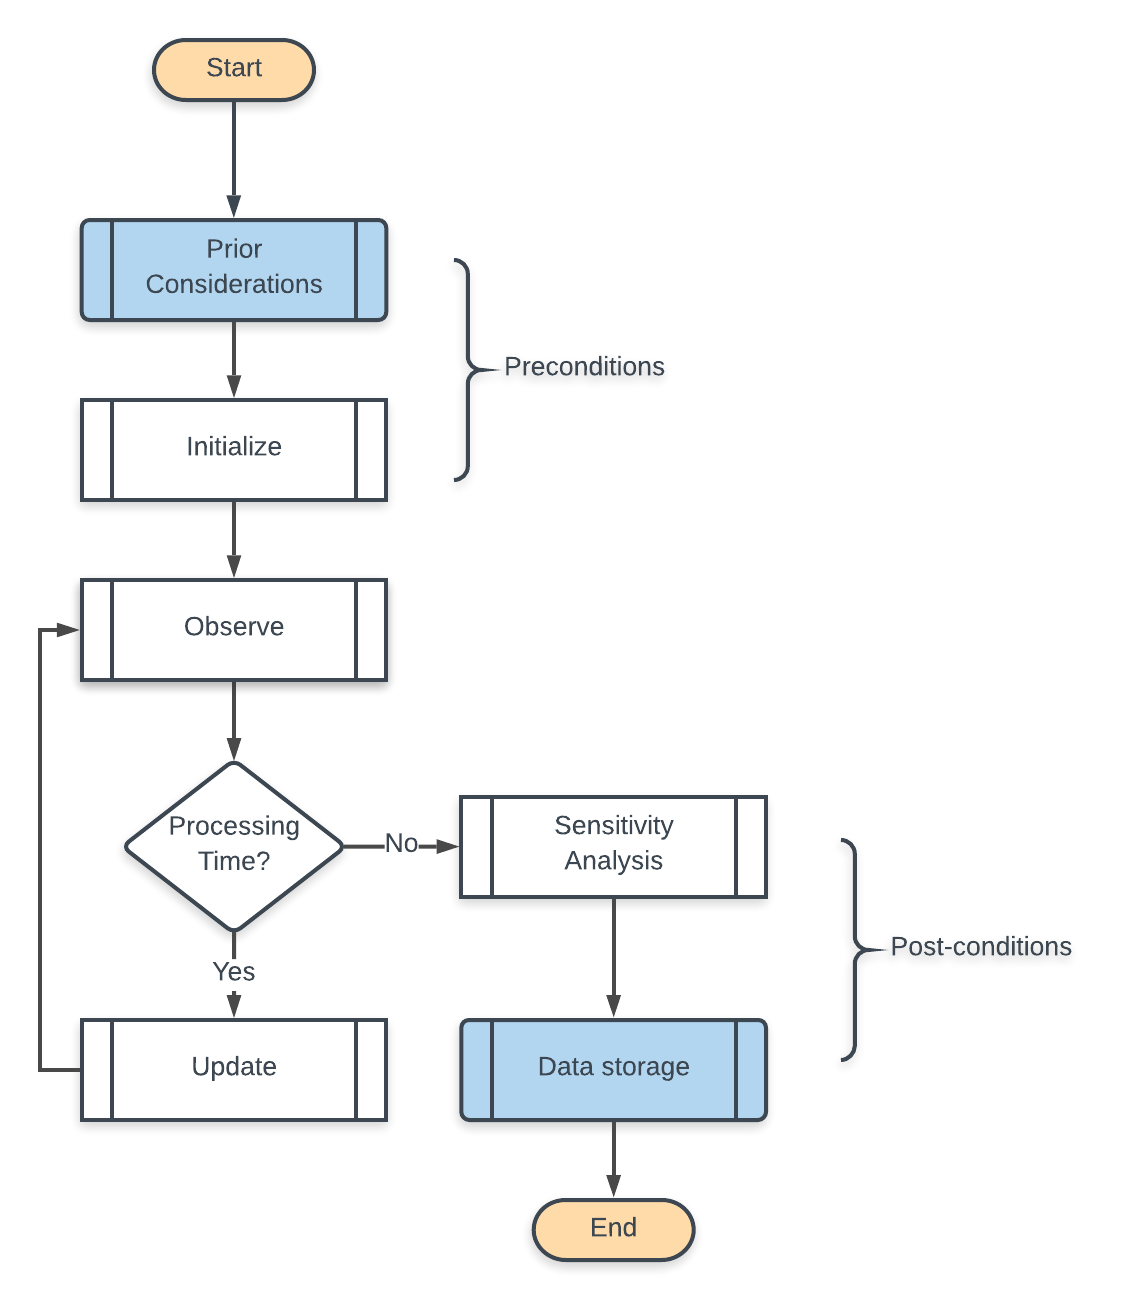
\includegraphics[scale=0.33]{workflow-scheme.png}
    \caption{Workflow diagram \\ (credits: made with \emph{Lucidchart})}
    \label{fig:workflow-scheme}
\end{figure}

\noindent
\textbf{Important}: Observe in Figure \ref{fig:workflow-scheme} the remaining steps categorized as \emph{Preconditions} and \emph{Postconditions}. They represent respectively the \emph{Before} and \emph{After} the 3 main steps \emph{Initialize, Observe, and Update} are executed. Note also that the \emph{Initialize} process is considered as part of the Preconditions semantics. That is because it only prepares the basic conditions for the components of the system, which are the habitats and the birds.

Analyzing the workflow diagram in Figure \ref{fig:workflow-scheme}, we denote the following fields:
\begin{itemize}
    \item \textbf{\textit{Start}}: indicates the starting point of the VE simulation.
    \item \textbf{\textit{Prior Considerations}}: are the basic setup necessary to fulfill the initialization phase requirements\footnote{These considerations, mostly based on the concerned entities (waterbirds, coastal lagoons), the environmental variables, and any additional properties contributing to the setup phase of the VE simulation, are also discussed in this document in the theoretical section.}. This setup spans the following elements: the geometry of the habitats and the human settlements; the functions defining the probability distribution of the random movements (driven by the water salinity, water depth, and food availability factors); the duration of the overall simulation process; and a reasonable threshold to handle the feasability of the random movements for a given seabird under certain conditions.
    \item \textbf{\textit{Initialize}}: creates the initial conditions of the system based on prior considerations mentioned above. That is, the patches (habitats) and agents (seabirds) creation.
    \item \textbf{\textit{Observe}}: generates a 2-dimensional plot whose scale goes from zero to one(\emph{$0-1$}) in both axes (x, y). The rendered plot helps to visualize both the patches' and agents' positions.
    \item \textbf{\textit{Processing Time?}}: focuses on updating the agents' positions' as long as the conditional parameter for the processing time holds. That is, the iteration is exclusively based on a specific number of times without accounting for other parameters that might influence the habitats and the birds. Note that, in this current version, the iteration is set statically during the prior considerations process.
    \item \textbf{\textit{Update}}: randomly assigns an agent to new positions within the existing habitats, considering a given threshold and the other aspects of the probability distribution.
    \item \textbf{\textit{Sensitivity Analysis}}: collects the probability values to form a set of probability distributions, which later can be analyzed and compared to each other with the expectation to draw conclusions on the final output.
    \item \textbf{\textit{Data Storage}}: given the generated plots, collects  them as PNG images and then generates a GIF out of the entire dumped images. This is relevant to provide the end-user useful insights on the collected data.
    \item \textbf{\textit{End}}: indicates the ending point of the VE simulation.
\end{itemize}

Recalling that this Virtual Environment constitutes essentially a digital representation of an Agent-Based Modeling system, each component of such a system relies on the interaction and interconnection with other involved components in an organized flow. Therefore, the diagram in Figure \ref{fig:workflow-scheme} shows a workflow scheme that intends to provide with a visual aid for a better understanding of the system's behaviour.

\subsection{Algorithm \& Data Structure}
The VE simulation implies the use of well-coordinated processes and subprocesses, which, once computed, will eventually attempt to explain the agents' behavior ant their mutual interactions with the environment in which they coexist. This section discusses the algorithm and data structure applied to contruct these processes and subprocesses.

\subsubsection{The \emph{Habitat} and \emph{Agent} data structure}
In the VE simulation, both the wetland areas and the human settlements of the coastal lagoons are represented by the term \emph{Habitat}\footnote{Note that human settlements are simply less appealing habitats for the waterbirds due to the humans' threatening characteristics}, and the waterbirds, by the term \emph{Agent}. In this case, the concept "Habitat"  is a 2-dimensional \emph{static} polygonal shape drawn from certain given geometrical measurements (see Figure 2). Similarly, the concept "Agent" is simply the representation of the waterbirds with some of its characteristics or attributes.

\begin{figure}[h!]
    \centering
    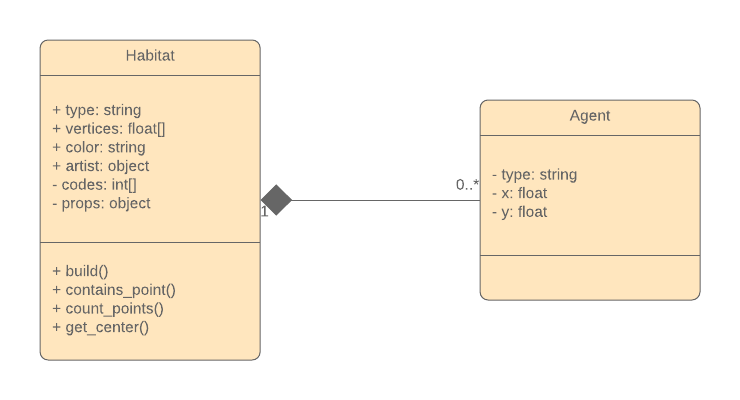
\includegraphics[scale=0.33]{data-structure.png}
    \caption{Data structure of \emph{Habitat} and \emph{Agent} \\ (credits: made with \emph{Lucidchart})}
    \label{fig:data-structure}
\end{figure}

\noindent
Observe that in Figure \ref{fig:data-structure} we use the class diagram named \emph{UML (Unified Modeling Language)} to model and document the properties of the components: Habitat and Agent. On the one hand, we construct a \textcolor{orange}{Habitat} class definition with the following properties:
\begin{itemize}
    \item \textbf{\textit{type}}: the type or category name of the habitat;
    \item \textbf{\textit{vertices}}: the coordinates of the patch representing the habitat;
    \item \textbf{\textit{color}}: the color (edge and face) to apply or distinguish a habitat from another;
    \item \textbf{\textit{artist}}: the patch-based polygonal shape to draw on a given figure;
    \item \textbf{\textit{props}}: the dictionary-like additional properties that characterize this habitat;
    \item \textbf{\textit{build()}}: constructs the \emph{artist} or patch on a figure;
    \item \textbf{\textit{contains\_point()}}: determines whether or not an x-y coordinate (point) belongs to a patch;
    \item \textbf{\textit{count\_points()}}: counts the total number of agents located within the patch based on their x-y positions.
    \item \textbf{\textit{get\_center()}}: obtains the center point (x-y coordinate)  of this habitat.
\end{itemize}

\noindent
On the other hand,  we construct an \textcolor{orange}{Agent} class definition with the following properties:
\begin{itemize}
    \item \textbf{\textit{type}}: the type or category name of the agent species;
    \item \textbf{\textit{x}}: the x-coordinate of the agent within an area;
    \item \textbf{\textit{y}}: the y-coordinate of the agent within an area.
\end{itemize}

\noindent
Keep in mind that some of the methods in the class definitions use helper functions to do their specific task. These helpers can be found in the Python scripts located in the Appendix section.

\subsubsection{The overall algorithm}
The overall algorithm is quite based on the step-by-step flow chart described in Figure \ref{fig:workflow-scheme}. In other words, it corresponds to the descriptive, logical aspects of the core functionality of the VE. The steps are as follows:

\begin{enumerate}
    \item \textbf{\textit{Given}}: given a collection of geometrical measurements (design) of the existing habitats and human settlements in a specific environment, a finite number (relatively small, 20 for example) of seabirds, and a set of predefined probability distribution functions (PDF) whose arguments are the characteristics of that environment;
    \item \textbf{\textit{Initialization}}: represent digitally (virtually) that environment by creating patches and agents;
    \item \textbf{\textit{Update}}: randomly choose an agent, then assess the probability of it moving to a random destination, and finally move the agent (if doable);
    \item \textbf{\textit{Observe}}: snapshot the current state of the plotted environment, then save figure as a PNG image;
    \item \textbf{\textit{Iterate}}: Repeat steps \textbf{3} \& \textbf{4} for $n$ times;
    \item \textbf{\textit{Stop}}: collect the dumped images and form GIF final image to visualize the random movements of the agents.
\end{enumerate}


\subsubsection{The \emph{Update} algorithm}
Some of the processes are really straightforward and do not demand a time-, or energy-consuming logic to build them. For instance, the initialization phase is one of the common cases where the developer only needs to take care of statically sets of values required as prior considerations for the initial conditions. But, as for the \emph{Update} process, a thoughtful, analytical solution is needed.

This algorithm basically defines an asynchronous approach to randomly update an agent's status, namely its geolocation. Thus, the set of instructions that follows below is the algorithm used to accomplish the "\emph{Synchronous Update}" functionality of the VE simulation:

\begin{enumerate}
    \item \textbf{\textit{Given}}: given a randomly selected agent;
    \item \textbf{\textit{Initialization}}: randomly choose a new destination within an "acceptable" habitat (an area where this agent can move to, given the environmental conditions);
    \item \textbf{\textit{Computation}}: compute the probability of that new destination use for this agent.
    \item \textbf{\textit{Update}}: finally, move the selected agent to that new destination if the calculated probability complies with the threshold.
\end{enumerate}

Recalling that this version of the project is a prototype whose purpose is to virtualize a static Agent-Based Modeling system, these algorithms are defined in their most simplistic mode. For this reason, they are subject to change in the future when it comes to updating the dynamics of the system or adding more complex variations.

\subsection{Implementation}
As mentioned in the \emph{Tools and Software} subsection in \emph{Instrumentation}, the VE simulation is implemented in a Jupyter Notebook workspace using the Python programming language. They are many reasons for choosing this particular setting to develop this workspace and the free cost is one of them.

The code implementation is based on the flow diagram presented in Figure \ref{fig:workflow-scheme} as well as the algorithms and data structure described in the previous subsection. Here, we mostly focus on the coding procedure and the programming standards to facilitate other colloborators' contributions and support in the future.

A standard programming workflow, if it does not involve too much of team management, demands to follow a set of intended principles\footnote{Those principles vary among institutions. So far, there is not yet a clear proposed draft describing them. Therefore, following them remains subjective.} that takes a system from a development stage to a production stage. For instance, the code should be: \textit{architected, modular, standardized, structured, scalable, secure, performance-oriented, tested, testable, collaborative, time-estimated, documented, and so on}. These principles are very common among big tech companies' projects and can also be used for smaller, or startup projects.

Since this actual version of the VE simulation is an early prototype, we focus on following part of these principles so far. Among them, figure:
\begin{itemize}
    \item \textbf{\textit{architected}}: the overall system follows a series of well-planned, modularized, interconnected conceptual tasks describing the interaction of the components within the system;
    \item \textbf{\textit{standardized}}: the script follows the rules for the naming conventions in Python (variable names, function and class definition, etc);
    \item \textbf{\textit{structured}}: the script is written semantically and logically, and organized sequentially (3rd-party libraries import, constants declaration, functions definition, and \emph{main}\footnote{Main entry function to run an application});
    \item \textbf{\textit{scalable}}: the script can be easily extended for new releases and anticipates enhancements in the future;
    \item \textbf{\textit{collaborative}}: the code is version-controlled using Git and GitHub online hosting service;
    \item \textbf{\textit{documented}}: the script is well-documented and describes the coding content in a very human-friendly way.
\end{itemize}

Besides the coding procedure, we also created a commonly-standardized, organized file structure (See Figure \ref{fig:file-structure}) for the project. Note the parent folders named \textit{\textcolor{blue}{src}} and \textit{\textcolor{blue}{docs}}. The former is for the source code of the project and the latter, for the documentation. The contents under those folders are backed-up and synced with an online GitHub repository for versioning and collaboration reasons.

Writing test is currently out of the scope of this release. We understand that using \emph{Unit Testing} and \emph{Integration Testing} for the implemented code is relatively important and should be covered. For now, the code is maintained and tested throughout the outputs and the visualizations as expected. But as for future updates or releases, the new implementation should be written using test-driven scripts methodology as the scalability of the project will make the code cumbersome to maintain and test.

\begin{figure}[h!]
    \centering
    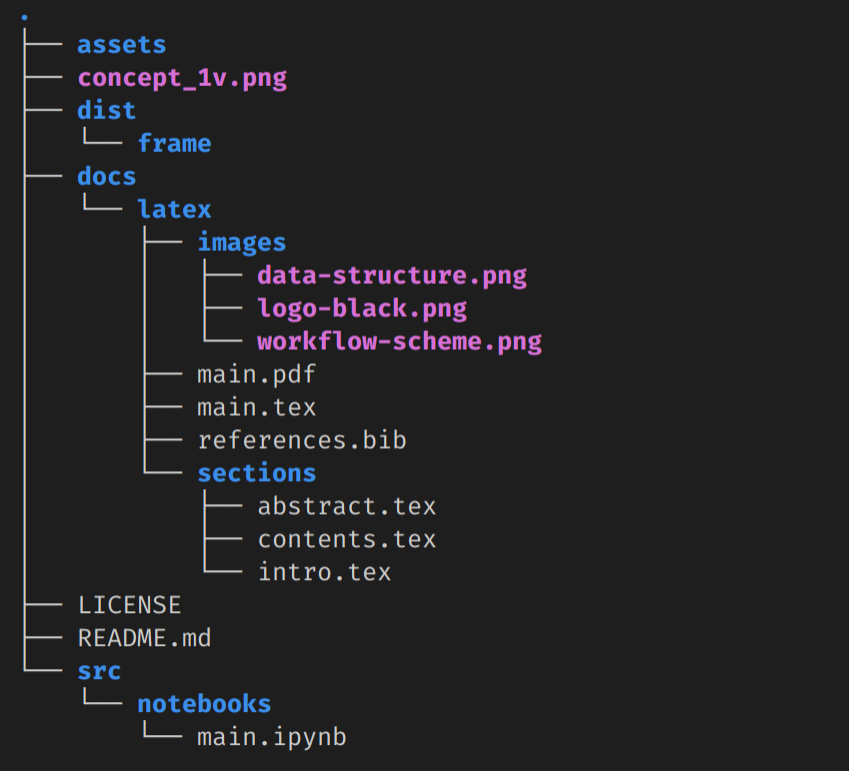
\includegraphics[scale=0.33]{file-structure.png}
    \caption{File structure of the project}
    \label{fig:file-structure}
\end{figure}

\subsection{Third-Party Libraries}

\subsubsection{Usage}
\subsubsection{Options}

\section{Results \& Discussions}

\section{Conclusion}

% ==============================================================================
% END: Methods, Results, Discussions, Conclusion
% ==============================================================================